\documentclass[10pt]{article}
\usepackage[margin=1in]{geometry}
\usepackage[T1]{fontenc}
\usepackage{lmodern}
\usepackage{amsmath}
\usepackage{booktabs}
\usepackage{graphicx}
\usepackage{xcolor}
\usepackage[numbers,sort&compress]{natbib}
\usepackage[hidelinks]{hyperref}
\usepackage{textcomp}
\usepackage{caption}
\captionsetup{font=small}

% Condition labels
\newcommand{\condI}{C1}
\newcommand{\condII}{C2}
\newcommand{\condIII}{C3}
\newcommand{\condIV}{C4}
\newcommand{\condVz}{C4$_0$}
\newcommand{\condV}{C5}
\newcommand{\todo}[1]{\textcolor{red}{[TODO: #1]}}

% 자동 생성: paper/make_assets.py — 직접 고치지 말 것
\newcommand{\bothMean}{\textminus0.2}
\newcommand{\bothPone}{0.53}
\newcommand{\bothPos}{6}
\newcommand{\corrHi}{18.2}
\newcommand{\corrLo}{\textminus1.6}
\newcommand{\corrMean}{+7.8}
\newcommand{\corrN}{5}
\newcommand{\corrPone}{0.031}
\newcommand{\corrPtwo}{0.0625}
\newcommand{\depthOpenflatCam}{+1.0}
\newcommand{\depthOpenflatLow}{+0.1}
\newcommand{\depthOpentiltCam}{+4.4}
\newcommand{\depthOpentiltLow}{+2.1}
\newcommand{\depthPinchflatCam}{+4.3}
\newcommand{\depthPinchflatLow}{+0.8}
\newcommand{\depthPinchtiltCam}{+10.2}
\newcommand{\depthPinchtiltLow}{+12.3}
\newcommand{\depthhumanHi}{20.0}
\newcommand{\depthhumanLo}{\textminus0.7}
\newcommand{\depthhumanMean}{+9.3}
\newcommand{\depthhumanN}{3}
\newcommand{\depthvirtHi}{\textminus3.3}
\newcommand{\depthvirtLo}{\textminus12.0}
\newcommand{\depthvirtMean}{\textminus7.3}
\newcommand{\depthvirtN}{3}
\newcommand{\doseOne}{70.3}
\newcommand{\doseTwo}{58.7}
\newcommand{\doseZero}{88.0}
\newcommand{\doseZeropFive}{87.3}
\newcommand{\graspPlaceThree}{3.8}
\newcommand{\graspPlaceTwo}{7.6}
\newcommand{\graspStackThree}{2.6}
\newcommand{\graspStackTwo}{3.2}
\newcommand{\jumpBase}{9.9}
\newcommand{\jumpCorr}{5.6}
\newcommand{\lossHi}{\textminus5.0}
\newcommand{\lossLo}{\textminus29.7}
\newcommand{\lossMean}{\textminus16.7}
\newcommand{\lossN}{3}
\newcommand{\lossShortHi}{\textminus21.8}
\newcommand{\lossShortLo}{\textminus44.0}
\newcommand{\lossShortMean}{\textminus32.8}
\newcommand{\markervscorrHi}{11.0}
\newcommand{\markervscorrLo}{\textminus9.3}
\newcommand{\markervscorrMean}{+0.3}
\newcommand{\markervscorrN}{3}
\newcommand{\outAnyPlace}{37.0}
\newcommand{\outAnyStack}{63.1}
\newcommand{\outPlace}{19.6}
\newcommand{\outStack}{56.5}
\newcommand{\pipelineHi}{8.7}
\newcommand{\pipelineLo}{1.0}
\newcommand{\pipelineMean}{+4.0}
\newcommand{\pipelineN}{3}
\newcommand{\ptwoThree}{54.4}
\newcommand{\ptwoTwo}{54.0}
\newcommand{\rangeBase}{10.3}
\newcommand{\rangeCorr}{4.2}
\newcommand{\recPlaceThreeMed}{28.9}
\newcommand{\recPlaceThreeTries}{53}
\newcommand{\recPlaceTwoMed}{25.5}
\newcommand{\recPlaceTwoTries}{51}
\newcommand{\recStackThreeMed}{16.3}
\newcommand{\recStackThreeTries}{60}
\newcommand{\recStackTwoMed}{14.6}
\newcommand{\recStackTwoTries}{57}
\newcommand{\residualHi}{\textminus0.3}
\newcommand{\residualLo}{\textminus14.0}
\newcommand{\residualMean}{\textminus7.3}
\newcommand{\residualN}{3}
\newcommand{\srFivelong}{85.3}
\newcommand{\srFiveshort}{59.4}
\newcommand{\srFourZerolong}{96.7}
\newcommand{\srFourZeroshort}{87.4}
\newcommand{\srFourlong}{89.3}
\newcommand{\srFourshort}{72.2}
\newcommand{\srOnelong}{92.7}
\newcommand{\srOneshort}{80.8}
\newcommand{\srThreelong}{84.4}
\newcommand{\srThreeshort}{60.4}
\newcommand{\srTwolong}{76.6}
\newcommand{\srTwoshort}{48.0}
\newcommand{\stackCorrHi}{1.0}
\newcommand{\stackCorrLo}{\textminus17.4}
\newcommand{\stackCorrMean}{\textminus8.2}
\newcommand{\stackDiscThree}{57}
\newcommand{\stackDiscTwo}{98}
\newcommand{\stackOne}{81.0}
\newcommand{\stackPone}{0.97}
\newcommand{\stackPos}{1}
\newcommand{\stackPtwo}{0.125}
\newcommand{\stackThree}{78.6}
\newcommand{\stackTwo}{86.8}
\newcommand{\stageThreeFloor}{81}
\newcommand{\stageThreeNolift}{2}
\newcommand{\stageThreeOnbase}{24}
\newcommand{\stageThreeSucc}{393}
\newcommand{\stageTwoFloor}{56}
\newcommand{\stageTwoNolift}{6}
\newcommand{\stageTwoOnbase}{4}
\newcommand{\stageTwoSucc}{434}


\title{How Much Does Monocular Depth Error Cost Imitation Learning?\\
\large Webcam Hand Teleoperation of a Simulated SO-101 Arm, with a Pre-registered Replication}
\author{\todo{author name}\\ Inha University\\ \texttt{kheechan04@gmail.com}}
\date{\todo{date}}

\begin{document}
\maketitle

\begin{abstract}
Collecting robot demonstrations with nothing but a laptop webcam is cheap, but a single camera must infer hand depth from apparent hand size, and that estimate is biased by hand pose.
We measure what this error does to imitation learning.
A human operator teleoperates a simulated SO-101 arm in MuJoCo from a webcam using MediaPipe hand landmarks, and ACT policies are trained on the resulting demonstrations.
On a pick-and-place task we compare six demonstration sources: scripted, webcam, webcam with a learned pose-dependent depth correction, a virtual operator running the same teleoperation code with and without injected measured depth error, and webcam with a wrist fiducial marker that measures depth directly.
With training length matched, webcam demonstrations yield \lossMean{} percentage points (pp) lower success than scripted ones (95\% CI [\lossLo, \lossHi]); at a fixed, shorter training length the gap appears twice as large (\lossShortMean{}~pp).
Injecting only the measured depth error into otherwise identical virtual-operator demonstrations lowers success in every seed (\depthvirtMean{}~pp, CI [\depthvirtLo, \depthvirtHi]), and success falls monotonically as the error is scaled up.
A CPU-only correction improved success on the placing task (\corrMean{}~pp over five seeds, exploratory), but a replication on a stacking task, with the analysis fixed before recording, did not reproduce it (\stackCorrMean{}~pp, CI [\stackCorrLo, \stackCorrHi]).
A post-hoc analysis suggests that the correction was applied outside the range of hand poses it was fitted on.
All code, 14 datasets and 35 trained policies are public.
\end{abstract}

% ---------------------------------------------------------------
\section{Introduction}

Low-cost arms such as the SO-100/101 are usually taught with a second ``leader'' arm that the operator moves by hand.
Hand tracking from an ordinary webcam would remove that hardware, and open-source pipelines that go from webcam hand tracking to simulated teleoperation to ACT~\citep{zhao2023act} training already exist~\citep{handrobot}.
The weak link is depth: with one camera, distance to the hand must be inferred from the hand's apparent size, and the hand's apparent size changes with its pose.

Prior work has shown that monocular teleoperation is slower and less accurate than teleoperation with depth sensing~\citep{qin2023anyteleop,teleopbench2025}, and in surgical robotics, policies trained on demonstrations estimated from monocular video succeed less often than policies trained on ground-truth demonstrations~\citep{chen2025surgipose}.
Within the literature we searched (Section~\ref{sec:related}), we did not find a controlled measurement of how much of the imitation-learning loss from webcam hand demonstrations is due to depth error specifically, or a test of whether a lightweight correction recovers it on more than one task.

We ask three questions:
\begin{enumerate}
\item How much lower is the success rate of a policy trained on webcam demonstrations than of one trained on scripted demonstrations?
\item How much of that loss is due to depth error?
\item Does a lightweight, CPU-real-time depth correction recover it?
\end{enumerate}

Our contributions are measurements rather than a new method:
(i) a pose-by-distance measurement of webcam depth error against tape-measured ground truth, showing a consistent pose-dependent bias of about 10--12~cm for the grasping hand pose;
(ii) a set of controlled demonstration conditions that separate depth error from other properties of human demonstrations, including a virtual operator that replays measured depth error through the identical teleoperation code and a dose-response sweep;
(iii) evidence that matching training length changes the conclusion substantially;
(iv) a pre-registered replication on a second task, which did not reproduce the effect of the correction, reported as it came out.

% ---------------------------------------------------------------
\section{Related Work}
\label{sec:related}

\paragraph{Vision-based teleoperation.}
AnyTeleop~\citep{qin2023anyteleop} supports RGB-only operation and reports that a single RGB camera is slower and more error-prone than RGB-D in a teleoperation task.
TeleOpBench~\citep{teleopbench2025} compares four teleoperation modalities, including monocular hand tracking, across 30 simulated bimanual tasks and finds monocular tracking the slowest.
Both evaluate teleoperation performance; neither trains policies on the collected demonstrations.
\citet{chiche2026shadowing} teleoperate an SO-ARM101 with RGB-D hand tracking and inverse kinematics.
The handrobot project~\citep{handrobot} implements a webcam-to-MuJoCo-to-ACT pipeline for SO-101; its reported policy success rates come from scripted demonstrations, a deliberate choice that makes them reproducible without a camera.

\paragraph{Demonstration quality and modality.}
\citet{mandlekar2021robomimic} and \citet{belkhale2023dataquality} show that demonstration quality strongly affects imitation learning, and \citet{li2025modality} compare kinesthetic, VR and spacemouse demonstrations.
Webcam hand tracking was not among the compared modalities.

\paragraph{Monocular demonstrations and policy success.}
SurgiPose~\citep{chen2025surgipose} estimates surgical tool pose from monocular video and trains policies on the estimates; these succeed less often than policies trained on ground-truth kinematics, and the estimation error is largest along the depth axis.
They do not isolate the share of the loss due to depth error.

\paragraph{Monocular distance estimation.}
RootNet~\citep{moon2019rootnet} estimates a person's camera distance with a pinhole relation and multiplies it by a correction factor learned from the image.
Our correction follows the same structure for hands, using a handful of hand-pose features and a linear model so that it runs in real time on a laptop CPU.

\paragraph{Search scope.}
We traced the 487 unique papers citing three anchor works~\citep{li2025modality,qin2023anyteleop,belkhale2023dataquality} (searched 2026-10-03, re-checked 2026-10-07).
Citation databases may miss recent work, so ``we did not find'' should be read within that scope.

% ---------------------------------------------------------------
\section{System}

\paragraph{Simulation and task.}
We use the SO-101 model from MuJoCo Menagerie~\citep{zakka2022menagerie} in MuJoCo~\citep{todorov2012mujoco}.
In the placing task the robot picks a 3~cm cube and places it on a marked target.
Fifty fixed layouts are used for demonstrations and a disjoint set of 100 fixed layouts for evaluation.
Success is judged by a single tracker used everywhere (scripted demonstrations, teleoperation, datasets, policy evaluation): the cube must be lifted and set down within the target, must not be pushed more than 1~cm after touching down, and must remain for 0.5~s.
In the stacking task the target is the top of a 4~cm block, which must not be displaced by more than 1~cm.

\paragraph{Teleoperation.}
MediaPipe Hand Landmarker~\citep{zhang2020mediapipehands} runs on the laptop CPU at about 31~fps.
Hand depth is estimated with a pinhole model from the smaller of the palm's image length and width; lateral and vertical position follow from the image coordinates.
The robot follows relative hand motion (with a clutch that re-anchors the reference), mapped to an end-effector target and solved with inverse kinematics.
Common processing for all webcam conditions consists of exponential smoothing, a gate that ignores depth jumps above 10~cm per frame, and a gripper switch driven by the thumb--index distance ratio that requires three consecutive frames before switching.
Wrist roll is fixed.
Webcam video is never stored; datasets contain only simulation camera images re-rendered from logged states.

\paragraph{Policy.}
We train LeRobot~\citep{cadene2024lerobot} 0.6.1 ACT with its default configuration (ResNet-18 backbone, chunk size 100, learning rate $10^{-5}$), batch size 8.
Observations are six joint positions and two 128$\times$128 simulated cameras (front and wrist); actions are six joint targets at 30~Hz.
Cube and target positions are not given to the policy.
Each policy is evaluated on the same 100 held-out layouts with a 60~s episode limit, fixed before results were seen.

% ---------------------------------------------------------------
\section{Depth Error and Its Correction}

\paragraph{Measurement.}
With the camera fixed, the operator held the hand at 35, 45, 55 and 65~cm (tape-measured along the optical axis) in four poses (open/pinch $\times$ frontal/tilted by about 45$^\circ$) at two heights, twice, in shuffled order, plus lateral positions (70 steps in total).
Table~\ref{tab:depth} shows the mean signed error.
The pose used when reaching for the cube, a pinch with a tilted palm, is read \depthPinchtiltCam{} and \depthPinchtiltLow{}~cm too far on average, always in the same direction.
Because the teleoperation follows relative motion, a constant offset is harmless; what matters is that changing hand shape at a fixed distance moves the estimate, and therefore the robot, along the camera axis.

\begin{table}[t]
\centering
\caption{Mean signed depth error (cm, estimate $-$ truth) by hand pose and height, averaged over distances 35--65~cm.}
\label{tab:depth}
\begin{tabular}{lrr}
\toprule
Hand pose & camera height & low (15~cm) \\
\midrule
open, frontal & \depthOpenflatCam & \depthOpenflatLow \\
open, tilted & \depthOpentiltCam & \depthOpentiltLow \\
pinch, frontal & \depthPinchflatCam & \depthPinchflatLow \\
pinch, tilted & \depthPinchtiltCam & \depthPinchtiltLow \\
\bottomrule
\end{tabular}
\end{table}

\paragraph{Correction (\condIII).}
Following RootNet~\citep{moon2019rootnet}, we multiply the pinhole distance by a learned factor,
$d = d_\text{pinhole} \exp(\mathbf{w}^\top \mathbf{f} + b)$,
where $\mathbf{f}$ holds six per-frame features computed from MediaPipe output alone: log pinhole distance, thumb--index ratio, a palm-tilt feature, the palm normal's component toward the camera, and the horizontal and vertical image position.
The model is a ridge regression on $\log(d_\text{true}/d_\text{pinhole})$ fitted only on the first measurement session; the regularisation strength and the feature set were fixed before evaluation, and the factor is clipped to the range seen in fitting.
On a second, unseen session the shift caused by changing hand shape fell from \jumpBase{} to \jumpCorr{}~cm and the range of per-pose mean errors from \rangeBase{} to \rangeCorr{}~cm, with no increase in jitter.

\paragraph{Marker (\condV).}
A printed 50~mm ArUco marker~\citep{garrido2014aruco} on a card at the inner wrist gives depth directly.
Its per-pose mean error ranged from $-0.9$ to $+1.2$~cm across the same poses.

% ---------------------------------------------------------------
\section{Experimental Design}

\paragraph{Conditions.}
\begin{itemize}
\item \condI{} \emph{scripted}: a program that knows the cube and target positions.
\item \condII{} \emph{webcam}: the operator teleoperates with uncorrected depth.
\item \condIII{} \emph{webcam + correction}: identical to \condII{} except that the correction is on.
\item \condVz{} and \condIV{} \emph{virtual operator}: a program that moves a virtual hand toward the same waypoints as \condI{}, watching the simulated gripper and correcting as a person would, fed through the identical teleoperation code.
In \condIV{} the hand depth carries measured error: the pose-dependent bias predicted from the hand-pose features of the human \condII{} demonstration on the same layout, plus that demonstration's frame-to-frame jitter. \condVz{} uses the true depth.
\item \condV{} \emph{webcam + marker}: the operator teleoperates with marker depth.
\end{itemize}
\condIV{} $-$ \condVz{} isolates depth error without a human; \condV{} $-$ \condII{} measures it within human demonstrations; \condV{} $-$ \condI{} is the loss that remains when depth is accurate.
A dose-response sweep scales the injected error by 0, 0.5, 1 and 2 (in log space, both bias and jitter); at scale 2 the virtual operator failed on 4 layouts, leaving 46 demonstrations.

\paragraph{Recording.}
Each condition has 50 demonstrations on the training layouts.
The operator (the author) recorded \condII{} and \condIII{} in alternating blocks to balance practice effects, and the condition was not shown on screen.
At recording time, \condII{} and \condIII{} did not differ: all 50 layouts were completed in both, with \recPlaceTwoTries{} and \recPlaceThreeTries{} attempts and a median of \recPlaceTwoMed{} and \recPlaceThreeMed{}~s to success.
\condV{} was recorded on the following day, interleaved with 20 additional \condII{} demonstrations that were used only to check for a change in operator skill and are not in the training data.

\paragraph{Exploratory and confirmatory stages.}
The placing-task experiments were exploratory: seeds were added once for \condII{} and \condIII{}, and the training length was extended to 100k steps after seeing that webcam conditions were under-trained.
Appendix~\ref{app:posthoc} lists every addition made after seeing results.
To test the one effect that remained uncertain, the correction, we then ran a replication on a new task with the plan fixed and committed before recording (Section~\ref{sec:stack}).

\paragraph{Statistics.}
All comparisons are paired by training seed.
Confidence intervals are 95\% percentile bootstrap intervals over 5,000 joint resamples of seeds and evaluation layouts.
For the correction we also report an exact sign-flip test over seeds; with five seeds the smallest possible two-sided $p$ is 0.0625.

% ---------------------------------------------------------------
\section{Results on the Placing Task}

\begin{table}[t]
\centering
\caption{Successes out of 100 held-out layouts. 20k steps: five seeds for every condition. 100k steps: five seeds for \condII{} and \condIII{}, three for the others.}
\label{tab:main}
\small
\begin{tabular}{lrrrr}
\toprule
 & \multicolumn{2}{c}{20k steps} & \multicolumn{2}{c}{100k steps} \\
\cmidrule(lr){2-3}\cmidrule(lr){4-5}
Condition & per seed & mean & per seed & mean \\
\midrule
\condVz{} virtual, no depth error & 86, 91, 87, 89, 84 & 87.4 & 96, 97, 97 & 96.7 \\
\condI{} scripted & 80, 73, 77, 91, 83 & 80.8 & 94, 90, 94 & 92.7 \\
\condIV{} virtual + depth error & 77, 65, 69, 77, 73 & 72.2 & 88, 90, 90 & 89.3 \\
\condV{} webcam + marker & 71, 46, 58, 61, 61 & 59.4 & 88, 86, 82 & 85.3 \\
\condIII{} webcam + correction & 68, 66, 64, 72, 32 & 60.4 & 80, 86, 89, 87, 80 & 84.4 \\
\condII{} webcam & 54, 37, 57, 55, 37 & 48.0 & 79, 84, 65, 79, 76 & 76.6 \\
\bottomrule
\end{tabular}

\end{table}

\begin{table}[t]
\centering
\caption{Paired comparisons at 100k steps (pp, successes out of 100). Only seeds present for both conditions are paired.}
\label{tab:comp}
\small
\begin{tabular}{llllr}
\toprule
Comparison & & per seed & mean & 95\% CI \\
\midrule
Webcam loss & \condII{} $-$ \condI{} & \textminus15, \textminus6, \textminus29 & \textminus16.7 & [\textminus29.7, \textminus5.0] \\
Depth error alone (no human) & \condIV{} $-$ \condVz{} & \textminus8, \textminus7, \textminus7 & \textminus7.3 & [\textminus12.0, \textminus3.3] \\
Depth share in human demos & \condV{} $-$ \condII{} & +9, +2, +17 & +9.3 & [\textminus0.7, 20.0] \\
Residual human-demo loss & \condV{} $-$ \condI{} & \textminus6, \textminus4, \textminus12 & \textminus7.3 & [\textminus14.0, \textminus0.3] \\
Effect of the teleop pipeline & \condVz{} $-$ \condI{} & +2, +7, +3 & +4.0 & [1.0, 8.7] \\
Correction (placing task) & \condIII{} $-$ \condII{} & +1, +2, +24, +8, +4 & +7.8 & [\textminus1.6, 18.2] \\
Marker vs.\ correction & \condV{} $-$ \condIII{} & +8, 0, \textminus7 & +0.3 & [\textminus9.3, 11.0] \\
\bottomrule
\end{tabular}

\end{table}

\paragraph{Training length changes the picture.}
Webcam demonstrations are much longer than scripted ones (median about 23--26~s vs.\ about 6~s), so at a fixed 20k steps a webcam demonstration is seen about 4 times versus 17.6 times for a scripted one.
At 20k steps webcam demonstrations looked \lossShortMean{}~pp worse than scripted (CI [\lossShortLo, \lossShortHi]).
At 100k steps (about 18 epochs for the webcam conditions) every condition improves (Table~\ref{tab:main}, Fig.~\ref{fig:length}) and the gap is \lossMean{}~pp (CI [\lossLo, \lossHi]).
Most of the apparent 20k-step loss was under-training.

\begin{figure}[t]
\centering
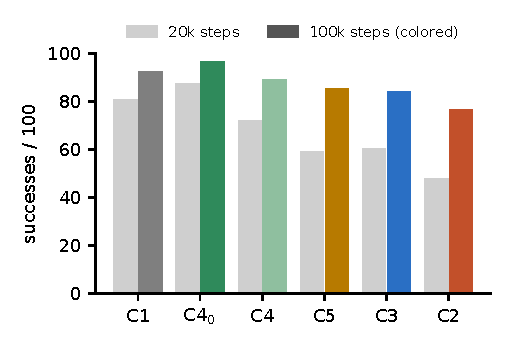
\includegraphics[width=0.48\linewidth]{figures/training_length.pdf}\hfill
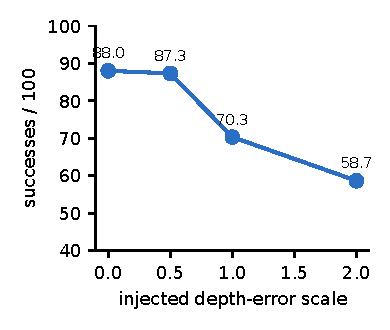
\includegraphics[width=0.40\linewidth]{figures/dose_response.pdf}
\caption{Left: mean successes at 20k and 100k steps. Right: virtual-operator success as the injected depth error is scaled (20k steps, three seeds).}
\label{fig:length}
\label{fig:dose}
\end{figure}

\paragraph{Depth error is a cause.}
With no human involved, injecting the measured depth error lowered success in all three seeds (\condIV{} $-$ \condVz{} = \depthvirtMean{}, CI [\depthvirtLo, \depthvirtHi]).
Scaling the error by 0, 0.5, 1 and 2 gave \doseZero, \doseZeropFive, \doseOne{} and \doseTwo{} successes (Fig.~\ref{fig:dose}).
In human demonstrations, measuring depth with the marker raised success by \depthhumanMean{}~pp over uncorrected webcam (\condV{} $-$ \condII, same direction in all three seeds, CI [\depthhumanLo, \depthhumanHi], touching zero).
A further \residualMean{}~pp (\condV{} $-$ \condI, CI [\residualLo, \residualHi]) remains when depth is accurate, which we attribute to other properties of human demonstrations.

\paragraph{The correction on the placing task.}
\condIII{} exceeded \condII{} in all five seeds (\corrMean{}~pp, CI [\corrLo, \corrHi]; sign-flip $p = \corrPtwo$ two-sided, \corrPone{} one-sided) and was at the level of the marker (\condV{} $-$ \condIII{} = \markervscorrMean).
A probe of where the trained policies first close the gripper showed a median front--back offset from the cube of \graspPlaceTwo{}~mm for \condII{} and \graspPlaceThree{}~mm for \condIII.

% ---------------------------------------------------------------
\section{Pre-registered Replication: Stacking}
\label{sec:stack}

Because the placing-task stage was exploratory and the correction's interval included zero, we did not add more seeds; we ran a new task instead.
Before recording, we fixed and committed: the task (red cube onto a 4~cm green block), 50 \condII{} and 50 \condIII{} demonstrations in alternating blocks with the condition hidden, the rule for setting training length (about 18 epochs, the same step count for \condII{} and \condIII), five seeds, a one-sided sign-flip test, a combined test with the placing task, and the verdict rule (\condIII{} better in 5/5 seeds: replicated; 4/5: mostly; 3 or fewer: not replicated), with no further seeds whatever the result.

Recording again showed no difference between conditions (\recStackTwoTries{} vs.\ \recStackThreeTries{} attempts for 50 successes; median \recStackTwoMed{} vs.\ \recStackThreeMed{}~s).
\condII{} and \condIII{} were trained for 60k steps and \condI{} for 20k.

\begin{table}[t]
\centering
\caption{Stacking task: successes out of 100 held-out layouts.}
\label{tab:stack}
\small
\begin{tabular}{llr}
\toprule
Condition & per seed & mean \\
\midrule
\condI{} scripted (20k) & 81, 79, 83 & 81.0 \\
\condII{} webcam (60k) & 86, 84, 88, 87, 89 & 86.8 \\
\condIII{} webcam + correction (60k) & 75, 87, 74, 82, 75 & 78.6 \\
\condIII{} $-$ \condII{} & \textminus11, +3, \textminus14, \textminus5, \textminus14 & \textminus8.2 \\
\bottomrule
\end{tabular}

\end{table}

\paragraph{Result.}
\condIII{} was better in \stackPos{} of 5 seeds (Table~\ref{tab:stack}); the mean difference was \stackCorrMean{}~pp (CI [\stackCorrLo, \stackCorrHi]; one-sided $p = \stackPone$).
Combining both tasks gives \bothMean{}~pp (one-sided $p = \bothPone$).
By the pre-registered rule, the effect was \textbf{not replicated}.
Across matched layouts, \condIII{} alone succeeded in \stackDiscThree{} episodes and \condII{} alone in \stackDiscTwo.

\begin{figure}[t]
\centering
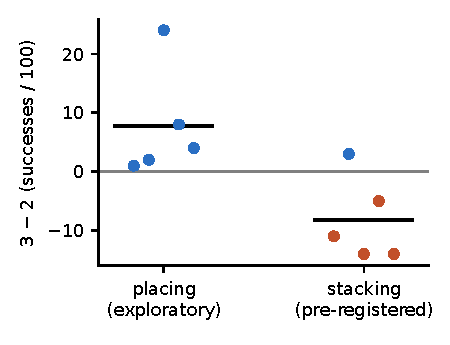
\includegraphics[width=0.42\linewidth]{figures/replication.pdf}
\caption{Per-seed difference \condIII{} $-$ \condII{} on each task; bars are means.}
\label{fig:rep}
\end{figure}

\paragraph{Post-hoc analyses (exploratory).}
These analyses were chosen after seeing the result and are hypotheses, not findings.
(i) Where policies failed: of 500 episodes per condition, \condII{} and \condIII{} succeeded in \stageTwoSucc{} and \stageThreeSucc; failures with the cube dropped or set on the floor numbered \stageTwoFloor{} and \stageThreeFloor, and failures with the cube on the block but not counted as success \stageTwoOnbase{} and \stageThreeOnbase.
Grasping was not worse with the correction (median front--back offset \graspStackTwo{} vs.\ \graspStackThree{}~mm for \condII{} and \condIII).
(ii) Range of the correction's inputs: in stacking, the hand was carried higher in the image to bring the cube above the block. The vertical image position was outside the range covered by the fitting data in \outStack\% of \condIII{} stacking frames versus \outPlace\% in placing, and at least one feature was outside in \outAnyStack\% versus \outAnyPlace\%.
A linear correction extrapolated outside its fitted range is a plausible reason for the reversal; testing it requires a new pre-registered study with a correction fitted over the stacking workspace.

% ---------------------------------------------------------------
\section{Discussion and Limitations}

Depth error from a webcam measurably lowers imitation-learning success, and its effect grows with its size.
A lightweight correction helped on one task and hurt on another, so we do not claim that it improves policies in general.
The comparison that changed most during the study was training length: equal step counts penalise long human demonstrations, and the 20k-step comparison roughly doubled the apparent loss.

Limitations:
\begin{itemize}
\item \emph{Operator.} The main operator is the author, who knew the hypothesis. The condition was hidden during recording and blocks alternated, but expectation effects cannot be excluded. A second demonstrator (20 \condII{} and 20 \condIII{} demonstrations, five seeds at 50k steps) showed no difference (\ptwoTwo{} vs.\ \ptwoThree{} successes); that person's depth bias was small, and the correction fitted to the first operator's hand added bias.
\item \emph{Scope.} Simulation only, two tasks, one camera, right hands.
\item \emph{Seeds.} Three to five seeds per condition; several intervals touch zero.
\item \emph{Exploratory analysis.} The placing-task stage involved decisions made after seeing results (Appendix~\ref{app:posthoc}); only the stacking replication was pre-registered.
\item \emph{Novelty.} The pipeline itself is not new~\citep{handrobot}; our contribution is the controlled measurement.
\end{itemize}

% ---------------------------------------------------------------
\section*{Data and Code Availability}
Code (Apache-2.0): \url{https://github.com/kheechan04/webcam-teach-robot}.
Datasets (CC BY 4.0) and the 35 final policies (Apache-2.0) are on the Hugging Face Hub under \texttt{kheechan04/webcam-teach-robot-*}.
All numbers, tables and figures in this paper are generated from the result files by \texttt{paper/make\_assets.py}.
The stacking plan is \texttt{docs/13-stacking-plan.md}, with its commit history.

\section*{Use of AI Tools}
An AI coding assistant (Claude Code, Anthropic) was used extensively throughout this project: it wrote most of the code and analysis scripts, proposed much of the experimental design and the analyses, and drafted the text of this paper.
The author performed all depth measurements, recorded all demonstrations of the primary operator, decided the direction of the study at key points (including stopping further seed additions and replicating on a new task with a pre-registered plan instead of running more experiments on the first task), reviewed the assistant's proposals and outputs, and takes full responsibility for the content.
All numbers, tables and figures are generated by scripts from the released result files. \todo{After checking: ``Every citation was checked against its source by the author.''}

\bibliographystyle{plainnat}
\bibliography{refs}

\appendix
\section{Additions Made After Seeing Results}
\label{app:posthoc}
Fixed before any result and never changed: the 100 evaluation layouts, the success tracker, the 60~s episode limit, the correction coefficients of \condIII{} (fitted on the first measurement session), and the recording rules (condition hidden, alternating blocks, at most three attempts per layout).

\begin{table}[h]
\centering
\small
\begin{tabular}{p{0.32\linewidth}p{0.28\linewidth}p{0.3\linewidth}}
\toprule
Addition & Reason & What it changed \\
\midrule
Seeds 3 $\to$ 5 at 20k steps (all conditions) & follow-up of first results & correction CI came to include zero \\
Depth-error scale 0.5 and 2 & is depth error causal? & success falls as error grows \\
Wrist marker (\condV) & does human correction of depth error add loss? & split loss into depth share and other human factors \\
100k steps for all conditions & webcam demos under-trained? & webcam loss 33 $\to$ 17~pp \\
Second demonstrator & does it hold for another person? & correction fitted to another hand had no effect \\
Seeds 3 $\to$ 5 at 100k for \condII, \condIII & correction effect borderline & $p = 0.0625$, still borderline; seed additions stopped and the question moved to the pre-registered stage \\
Stacking failure stages, grasp probe, feature range & understand the non-replication & hypothesis only (Section~\ref{sec:stack}) \\
\bottomrule
\end{tabular}
\end{table}

All results of added experiments are reported, including unfavourable ones. Adding seeds after seeing results risks optional stopping, which is why the placing-task correction effect is treated as borderline and the conclusion rests on the pre-registered replication.

\end{document}
